\chapter{HASIL YANG DIHARAPKAN}

\section{Hasil yang Diharapkan dari Penelitian}
Hasil yang diharapkan pada penelitian ini adalah dihasilkannya model Vision Transformer dapat melakukan re-identifikasi pada penyu penyu berdasarkan citra kepalanya dengan akurasi di atas 85\%.

\section{Hasil Pendahuluan}
Sampai saat ini, penelitian ini mendapatkan hasil berupa pencarian dataset yang nantinya akan diolah dan digunakan untuk pengembangan model Vision Transformer.
Dataset yang telah terkumpul antara adalah SeaTurtleIDHeads, SeaTurtleID2022, SeaTurtleID,
Dataset ini berupa citra kepala penyu yang didapatkan dari platform Kaggle dan Papers with Code.
\begin{figure} [H] \centering
    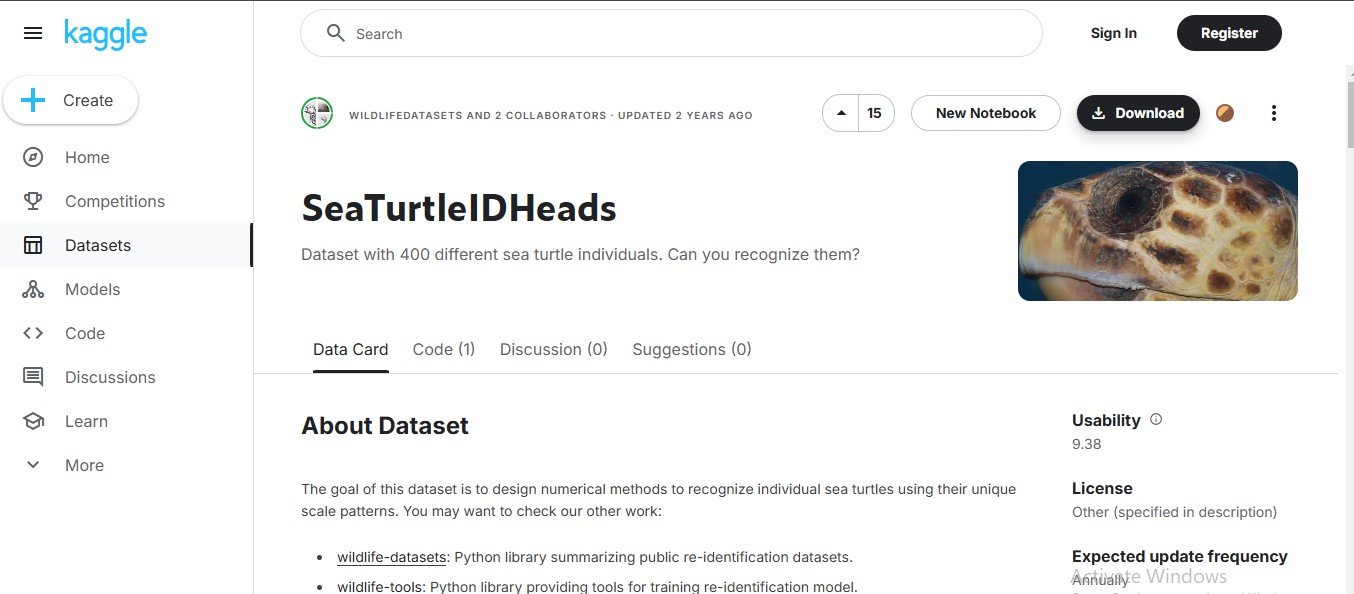
\includegraphics[scale=0.45]{gambar/SeaTurtleIDHeads.jpg}
    \caption{dataset SeaTurtleIDHeads}
    \label{fig:SeaTurtleIDHeads}
\end{figure}
\begin{figure} [H] \centering
    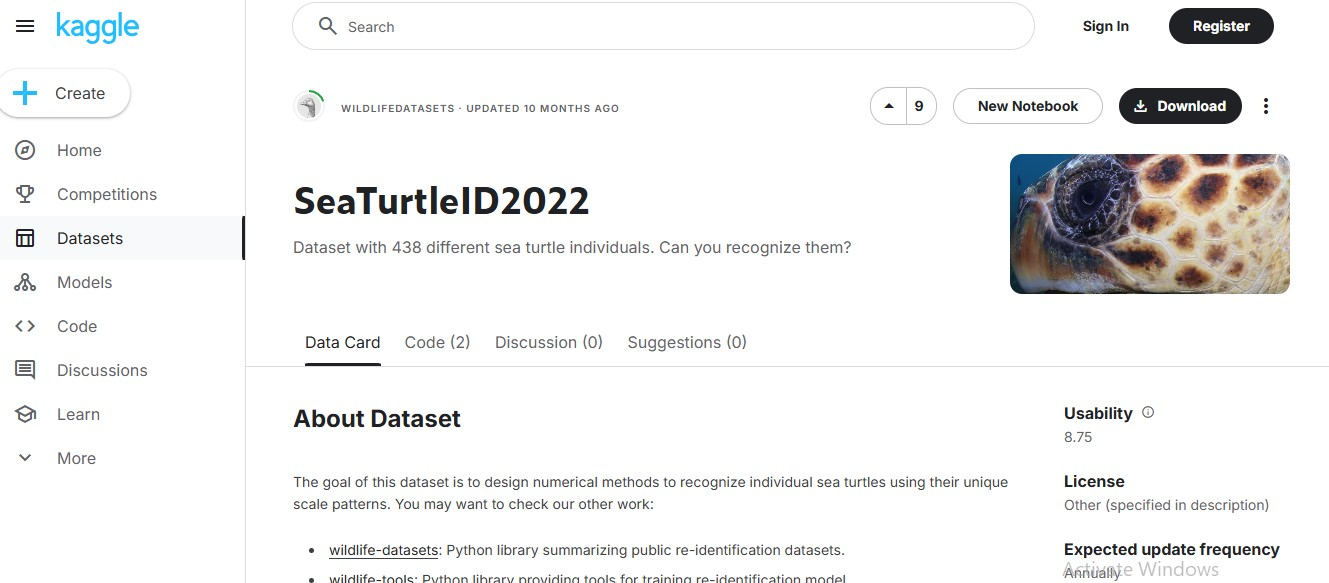
\includegraphics[scale=0.45]{gambar/SeaTurtleID2022.jpg}
    \caption{dataset SeaTurtleID2022}
    \label{fig:SeaTurtleID2022}
\end{figure}
\begin{figure} [H] \centering
    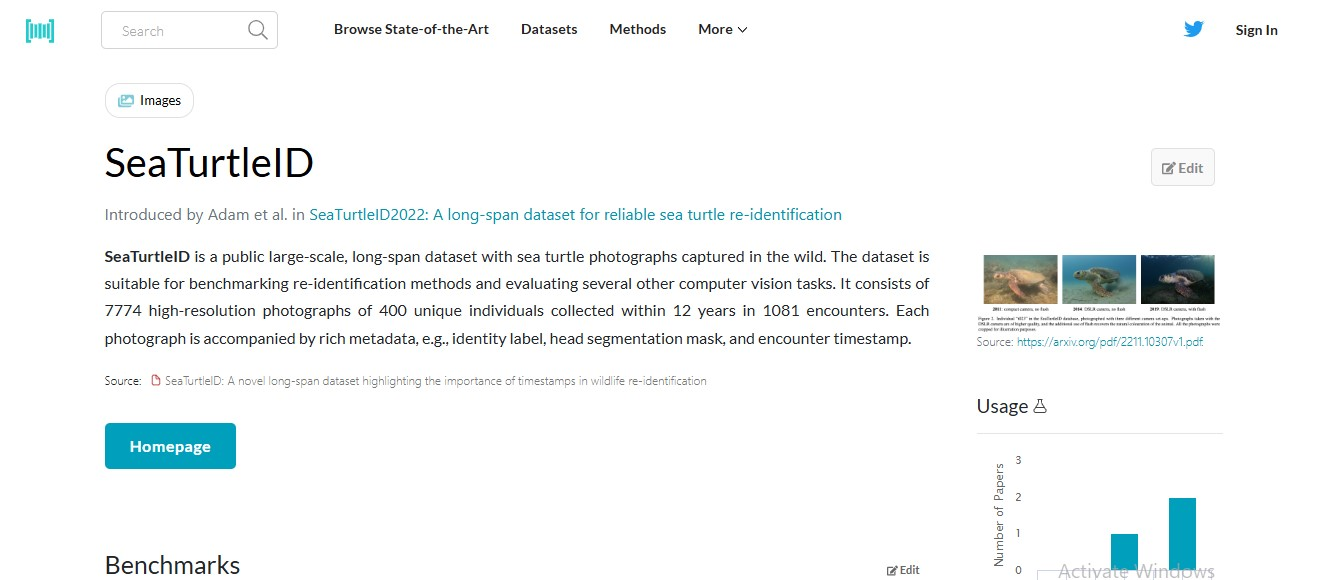
\includegraphics[scale=0.45]{gambar/SeaTurtleID.jpg}
    \caption{dataset SeaTurtleID}
    \label{fig:SeaTurtleID}
\end{figure}

Selain itu, penulis telah menemukan kumpulan dataset fauna yang dikhususkan untuk kebutuhan re-identifikasi yang bernama Wildlife Datasets.
Wildlife Datasets berupa package python yang dapat mengunduh dataset sesuai dengan katalog yang tersedia.
\begin{figure} [H] \centering
    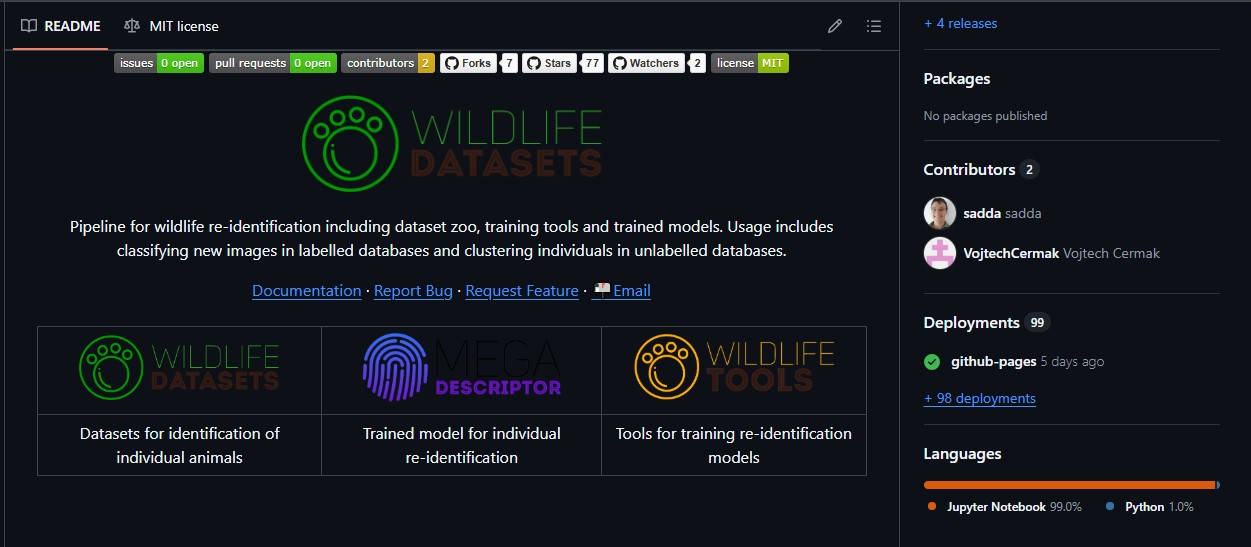
\includegraphics[scale=0.45]{gambar/Wildilfe.jpg}
    \caption{Wildlife Datasets}
    \label{fig:Wildlife}
\end{figure}

Penulis juga telah melakukan pengujian \textit{training} model Vision Transformer dengan menggunakan Pytorch dan torchvision.
\begin{figure} [H] \centering
    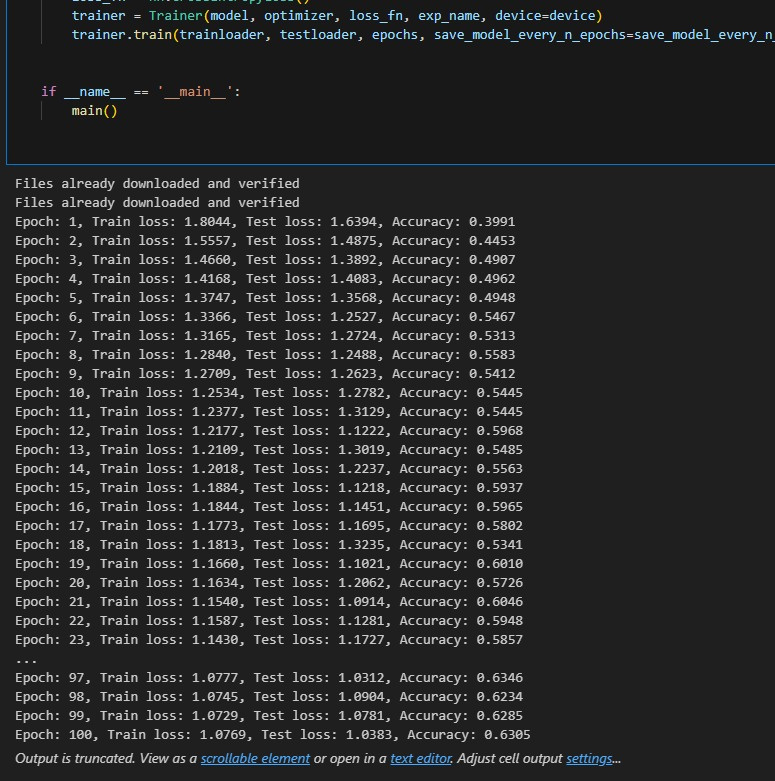
\includegraphics[scale=0.45]{gambar/training.jpg}
    \caption{Proses Training}
    \label{fig:Training}
\end{figure}
\begin{figure} [H] \centering
    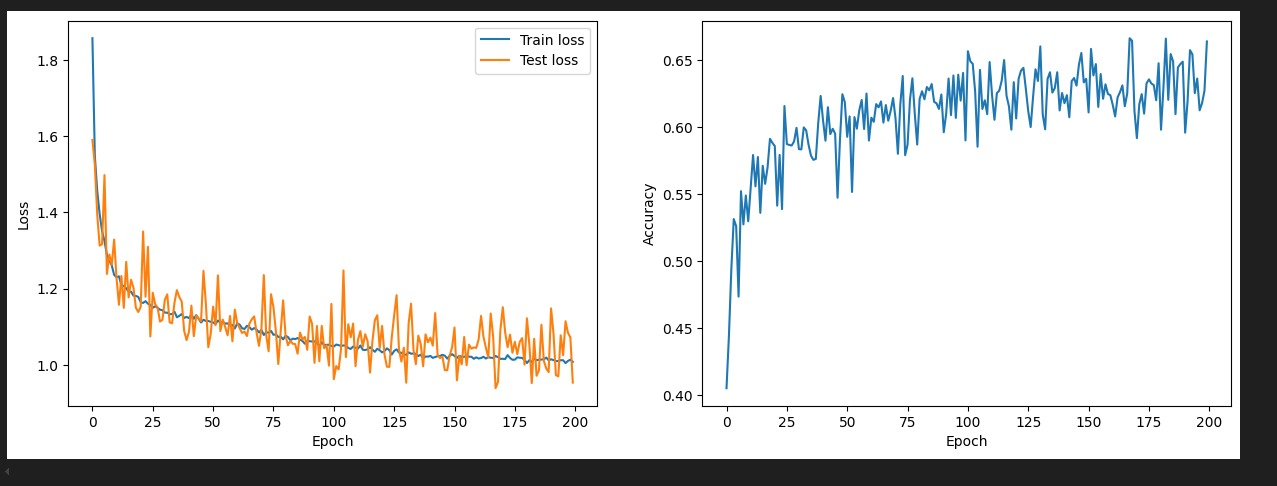
\includegraphics[scale=0.30]{gambar/graph.jpg}
    \caption{Grafik Akurasi}
    \label{fig:Graph}
\end{figure}
\begin{figure} [H] \centering
    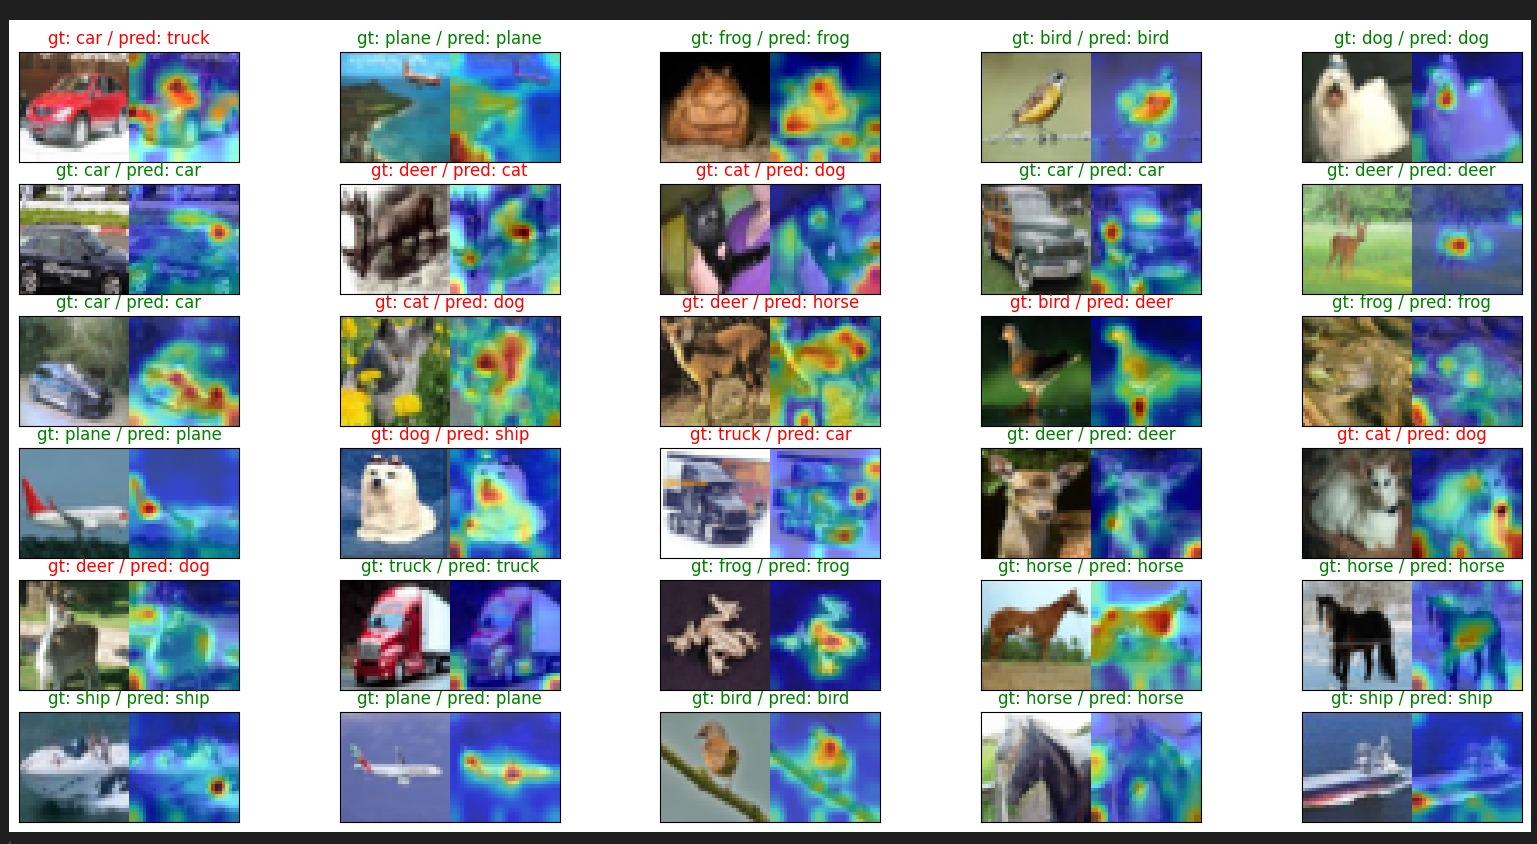
\includegraphics[scale=0.30]{gambar/test.jpg}
    \caption{Hasil Pengujian Identifikasi}
    \label{fig:Identification}
\end{figure}